% Provenance (never printed): see sources/outline_sources.md (Year 3:
% concordia and discordia; 40Ar/39Ar step heating; Sm-Nd model ages;
% cosmogenic nuclides; fission tracks and (U-Th)/He). Brief:
% sources/book5/BRIEFS.md, ch. 13. Curves from figdata/bachelor-3/
% concordia.py, arar_spectrum.py, model_ages.py, cosmogenic.py. Exercise and
% problem values in the Book 5 scratch calculator calc/ch13.py. The zircons,
% the biotite spectrum, the Nd sample and the helium ages of the Varden
% granite are invented, consistent with the Year 1 volume's granite of 310 Ma.
\chapter{Géochronologie avancée}\label{ch:b3:advanced-geochronology}

Un cristal de zircon long d'un dixième de millimètre entretient deux horloges en marche
depuis la cristallisation de son granite~: l'uranium-238 qui se désintègre en plomb-206 et
l'uranium-235 qui se désintègre en plomb-207. Quand les deux horloges concordent, l'âge
est hors de doute. Quand elles ne concordent pas, la discordance elle-même peut être datée~: le
cristal a perdu une partie de son plomb lors d'un événement ultérieur, et les deux
horloges, lues conjointement, donnent l'âge du granite et celui de l'événement. Ce chapitre
lit plusieurs horloges à la fois, dans l'uranium et le plomb, dans l'argon, dans le
néodyme, dans les traces de fission et l'hélium, et dans les rares atomes produits par
les rayons cosmiques, et il indique dans quelle mesure chaque âge est digne de confiance.

\begin{recall}
La désintégration radioactive, l'équation de l'âge, l'isochrone et son rapport initial, la
droite des moindres carrés, la désintégration à embranchement, l'âge potassium--argon,
la température de fermeture et l'âge de refroidissement figurent dans le volume de première
année, dans son chapitre sur la datation radiométrique~; la formule d'érosion stationnaire
des \omterm{def:b3:advanced-geochronology:cosmogenic}{nucléides cosmogéniques} se trouve dans son chapitre sur l'érosion et le transport. Le
réservoir uniforme chondritique, la notation epsilon et le manteau appauvri figurent dans le
volume de deuxième année, dans son chapitre sur la géochimie isotopique~; la spectrométrie
de masse à thermo-ionisation et la spectrométrie de masse multicollectrice, dans son chapitre sur les méthodes de terrain et de laboratoire. La
\omterm{def:b3:orogenic-wedges:thermochronology}{thermochronologie} et la \omterm{def:b3:orogenic-wedges:age-elevation}{relation âge--altitude} sont traitées au \cref{ch:b3:orogenic-wedges}.
\end{recall}

\section{Uranium, plomb et concordia}\label{sec:b3:advanced-geochronology:upb}

L'uranium possède deux isotopes à longue durée de vie. L'uranium-238 se désintègre par une chaîne
de descendants à courte durée de vie jusqu'au plomb-206 avec $\lambda_{238} =
\qty{1.55125e-10}{an^{-1}}$~; l'uranium-235 se désintègre en plomb-207 avec $\lambda_{235}
= \qty{9.8485e-10}{an^{-1}}$, six fois plus vite. Leur rapport actuel est
$^{235}\mathrm{U}/^{238}\mathrm{U} = 0.0072567$, soit $^{238}\mathrm{U}/^{235}\mathrm{U}
= 137.8$, le même dans toutes les roches terrestres. Le zircon, $\mathrm{ZrSiO_4}$, incorpore
beaucoup d'uranium et presque pas de plomb lors de sa croissance, et il résiste à l'altération
et survit au métamorphisme~: presque tout son plomb est radiogénique.
% ledger: amherst:constants, tulane:upb-zircon

Notons $x = {}^{207}\mathrm{Pb}^*/{}^{235}\mathrm{U}$ et $y =
{}^{206}\mathrm{Pb}^*/{}^{238}\mathrm{U}$ pour les rapports actuels du plomb radiogénique
à son élément père. Chacun donne un âge, $t_{206} = \ln(1 + y)/\lambda_{238}$
et $t_{207} = \ln(1 + x)/\lambda_{235}$.

\begin{definition}[Concordia, discordia, intercepts, diagramme de Tera--Wasserburg]
\label{def:b3:advanced-geochronology:concordia}
La \emph{concordia}\index{concordia} est la courbe du plan $(x, y)$ sur
lequel les deux âges uranium--plomb sont égaux. La \emph{discordia}\index{discordia}
est une droite le long de laquelle s'alignent les analyses discordantes d'une population
de cristaux~; ses intersections avec la concordia sont les
\emph{intercept supérieur}\index{intercept supérieur} (le plus ancien) et le
\emph{intercept inférieur}\index{intercept inférieur} (le plus jeune). Le
\emph{diagramme de Tera--Wasserburg}\index{diagramme de Tera--Wasserburg} représente
$X = {}^{238}\mathrm{U}/{}^{206}\mathrm{Pb}^*$ en fonction de $Y =
{}^{207}\mathrm{Pb}^*/{}^{206}\mathrm{Pb}^*$.
\end{definition}

\begin{theorem}[La concordia]\label{thm:b3:advanced-geochronology:concordia}
Un cristal resté clos à l'uranium et au plomb depuis sa formation, il y a
un temps $t$, se place en
\[
C(t) = \bigl(e^{\lambda_{235}t} - 1,\; e^{\lambda_{238}t} - 1\bigr).
\]
Lorsque $t$ croît, la courbe monte de plus en plus lentement par rapport à $x$~: sa pente,
$\mathrm dy/\mathrm dx = (\lambda_{238}/\lambda_{235})\,e^{(\lambda_{238} -
\lambda_{235})t}$, décroît depuis $\lambda_{238}/\lambda_{235} = 0.1575$ à
l'origine, donc la \omterm{def:b3:advanced-geochronology:concordia}{concordia} est concave vers l'axe des $x$.
\end{theorem}

\begin{proof}
Pour chaque élément père, le nombre de descendants radiogéniques par atome père restant est
$e^{\lambda t} - 1$, l'équation de l'âge du volume de première année. En dérivant
les deux coordonnées par rapport à $t$ et en divisant on obtient la pente~; comme
$\lambda_{235} > \lambda_{238}$, elle décroît avec $t$.
\end{proof}

Le plomb est un gros ion qui s'insère mal dans le réseau du zircon. Dans les parties
d'un cristal endommagées par sa propre radioactivité, le plomb peut en sortir lors
d'un événement ultérieur de chauffage ou de circulation de fluides.
% ledger: tulane:upb-zircon

\begin{theorem}[Une perte épisodique de plomb donne une corde]\label{thm:b3:advanced-geochronology:discordia}
Un cristal formé il y a un temps $t_1$, qui a perdu il y a un temps $t_2$, une fraction $f$
de son plomb radiogénique, et est resté clos par ailleurs, se place aujourd'hui en
\[
(1 - f)\,C(t_1) + f\,C(t_2),
\]
sur la corde joignant les points $t_1$ et $t_2$ de la \omterm{def:b3:advanced-geochronology:concordia}{concordia}. Les cristaux qui
ont perdu des fractions différentes sont alignés sur cette corde, une \omterm{def:b3:advanced-geochronology:concordia}{discordia} dont
l'\omterm{def:b3:advanced-geochronology:concordia}{intercept supérieur} est $t_1$ et l'\omterm{def:b3:advanced-geochronology:concordia}{intercept inférieur} est $t_2$.
\end{theorem}

\begin{proof}
Prenons un système de désintégration de constante $\lambda$, et comptons par atome parent
présent aujourd'hui. Il y a un temps $t_2$, il y avait $e^{\lambda t_2}$ atomes parents, et
descendants radiogéniques $e^{\lambda t_2}(e^{\lambda(t_1 - t_2)} - 1) =
e^{\lambda t_1} - e^{\lambda t_2}$. L'événement en a laissé $(1 - f)(e^{\lambda t_1} -
e^{\lambda t_2})$~; depuis, le parent en a produit $e^{\lambda t_2} - 1$ de plus. La
somme vaut $(1 - f)(e^{\lambda t_1} - 1) + f(e^{\lambda t_2} - 1)$. Les deux isotopes
du plomb se comportent de façon identique sur le plan chimique, si bien que $f$ vaut la même chose pour les deux, et
les deux coordonnées se combinent au point énoncé.
\end{proof}

\begin{omfigure}
\begin{tikzpicture}
\begin{groupplot}[group style={group size=2 by 1, horizontal sep=1.7cm},
  omrecord, width=0.47\linewidth, height=0.42\linewidth, title style={font=\small},
  tick label style={font=\scriptsize}, label style={font=\small}]
\nextgroupplot[title={(a) diagramme de concordia},
  xlabel={$^{207}\mathrm{Pb}^*/^{235}\mathrm{U}$}, ylabel={$^{206}\mathrm{Pb}^*/^{238}\mathrm{U}$},
  xmin=0.04, xmax=0.44, ymin=0.006, ymax=0.06,
  xtick={0.1,0.2,0.3,0.4}, xticklabels={0.1,0.2,0.3,0.4},
  ytick={0.01,0.02,0.03,0.04,0.05}, yticklabels={0.01,0.02,0.03,0.04,0.05},
  scaled ticks=false]
% computed in figdata/bachelor-3/concordia.py
\addplot[black, thick] table[x=xw, y=yw] {figdata/out/bachelor-3-concordia-curve.dat};
\addplot[black, only marks, mark=*, mark size=1.4pt, nodes near coords={\scriptsize\pgfmathprintnumber[fixed, precision=0]{\pgfplotspointmeta}},
  point meta=explicit, nodes near coords align={anchor=south east},
  restrict expr to domain={\thisrow{t}}{100:350}]
  table[x=xw, y=yw, meta=t] {figdata/out/bachelor-3-concordia-ticks.dat};
\addplot[omDef, thick, densely dashed] table[x=x, y=y] {figdata/out/bachelor-3-concordia-line.dat};
\addplot[red!70!black, only marks, mark=diamond*, mark size=2pt] table[x=x, y=y] {figdata/out/bachelor-3-concordia-zircons.dat};
\nextgroupplot[title={(b) diagramme de Tera--Wasserburg},
  xlabel={$^{238}\mathrm{U}/^{206}\mathrm{Pb}^*$}, ylabel={$^{207}\mathrm{Pb}^*/^{206}\mathrm{Pb}^*$},
  xmin=15, xmax=75, ymin=0.0465, ymax=0.0535,
  ytick={0.047,0.049,0.051,0.053}, yticklabels={0.047,0.049,0.051,0.053},
  scaled ticks=false]
\addplot[black, thick] table[x=xtw, y=ytw] {figdata/out/bachelor-3-concordia-curve.dat};
\addplot[black, only marks, mark=*, mark size=1.4pt, nodes near coords={\scriptsize\pgfmathprintnumber[fixed, precision=0]{\pgfplotspointmeta}},
  point meta=explicit, nodes near coords align={anchor=north east},
  restrict expr to domain={\thisrow{t}}{100:250}]
  table[x=xtw, y=ytw, meta=t] {figdata/out/bachelor-3-concordia-ticks.dat};
\addplot[omDef, thick, densely dashed] table[x=xtw, y=ytw] {figdata/out/bachelor-3-concordia-twline.dat};
\addplot[red!70!black, only marks, mark=diamond*, mark size=2pt] table[x=xtw, y=ytw] {figdata/out/bachelor-3-concordia-zircons.dat};
\end{groupplot}
\end{tikzpicture}

\par\smallskip{\small (a) La \omterm{def:b3:advanced-geochronology:concordia}{concordia}, avec ses âges en millions d'années,
et cinq zircons discordants fictifs d'un même granite (en rouge~; leurs
ellipses d'erreur sont plus petites que les symboles), alignés sur une \omterm{def:b3:advanced-geochronology:concordia}{discordia} (en tirets) qui
recoupe la \omterm{def:b3:advanced-geochronology:concordia}{concordia} près de 311 et \qty{100}{\Ma}. (b) Les mêmes zircons et la
même droite dans le \omterm{def:b3:advanced-geochronology:concordia}{diagramme de Tera--Wasserburg}, où une \omterm{def:b3:advanced-geochronology:concordia}{discordia} reste une
droite.}\label{fig:b3:advanced-geochronology:concordia}
\end{omfigure}
% ledger: amherst:constants

Les intercepts se trouvent là où $a + b\,x(t) = y(t)$, équation en $t$ qui se résout
par la méthode de Newton~: avec $g(t) = e^{\lambda_{238}t} - 1 - a -
b(e^{\lambda_{235}t} - 1)$ et $g'(t) = \lambda_{238}e^{\lambda_{238}t} -
b\lambda_{235}e^{\lambda_{235}t}$, on itère $t \leftarrow t - g/g'$ à partir d'une estimation
voisine de chaque intercept. Trois propriétés du résultat comptent en pratique.
D'abord, l'\omterm{def:b3:advanced-geochronology:concordia}{intercept supérieur} n'est précis que si la \omterm{def:b3:advanced-geochronology:concordia}{discordia} recoupe la
\omterm{def:b3:advanced-geochronology:concordia}{concordia} sous un grand angle. Une \omterm{def:b3:advanced-geochronology:concordia}{discordia} jeune, comme sur la figure ci-dessus, court
presque le long de la \omterm{def:b3:advanced-geochronology:concordia}{concordia}, et une petite variation de sa pente déplace
l'intercept très loin. Ensuite, si la perte de plomb est récente, $t_2 = 0$, la
\omterm{def:b3:advanced-geochronology:concordia}{discordia} passe par l'origine, et chaque cristal a le même
rapport $^{207}\mathrm{Pb}^*/^{206}\mathrm{Pb}^*$,
\[
\frac{^{207}\mathrm{Pb}^*}{^{206}\mathrm{Pb}^*} = \frac{1}{137.8}\,
\frac{e^{\lambda_{235}t_1} - 1}{e^{\lambda_{238}t_1} - 1},
\]
ce qui donne $t_1$ sans l'uranium~: l'âge plomb--plomb. Enfin, une droite du
diagramme \omterm{def:b3:advanced-geochronology:concordia}{concordia}, $x = (y - a)/b$, devient dans les
coordonnées de Tera--Wasserburg $Y = (1 - aX)/(137.8\,b)$, à nouveau une droite. Le
\omterm{def:b3:advanced-geochronology:concordia}{diagramme de Tera--Wasserburg} utilise des rapports mesurés directement, sans qu'il faille calculer
l'uranium-235 à partir de l'uranium-238, et un mélange avec du plomb commun, non radiogénique et riche en
plomb-207, se place sur une droite qui coupe l'axe $Y$ au rapport du plomb
commun.

Les âges uranium--plomb se mesurent de deux façons. Des cristaux isolés ou des
fragments, dissous après que les zones endommagées ont été éliminées par une
dissolution partielle et que leur plomb et leur uranium ont été séparés, se mesurent par
spectrométrie de masse à thermo-ionisation, qui donne les âges les plus précis de la géologie. Des spots de quelques dizaines de
micromètres de diamètre se mesurent sur place, à la microsonde ionique ou par
ablation laser, de façon moins précise mais zone par zone à travers un cristal qui a
crû au cours de plusieurs événements.

\begin{inthelab}[Le laboratoire de géochronologie]
\begin{minipage}[t]{0.55\linewidth}\vspace{0pt}
Une datation sur zircon commence avec une roche broyée et se termine dans un laboratoire propre. Les
géochronologues séparent les zircons par densité et magnétisme, sélectionnent les
cristaux les plus nets au microscope binoculaire et photographient leur zonation. Les
cristaux sont partiellement dissous pour éliminer leurs zones endommagées, puis dissous
entièrement avec un traceur d'isotopes connus, et l'uranium et le plomb sont
séparés sur de minuscules colonnes de résine, dans un air filtré pour écarter le plomb
des poussières. Un spectromètre de masse mesure les rapports isotopiques. Les échantillons d'argon suivent un
autre chemin~: un réacteur, puis une ligne à gaz où un laser chauffe chaque palier et
où l'argon est épuré avant le spectromètre.
\end{minipage}\hfill
\begin{minipage}[t]{0.42\linewidth}\vspace{0pt}
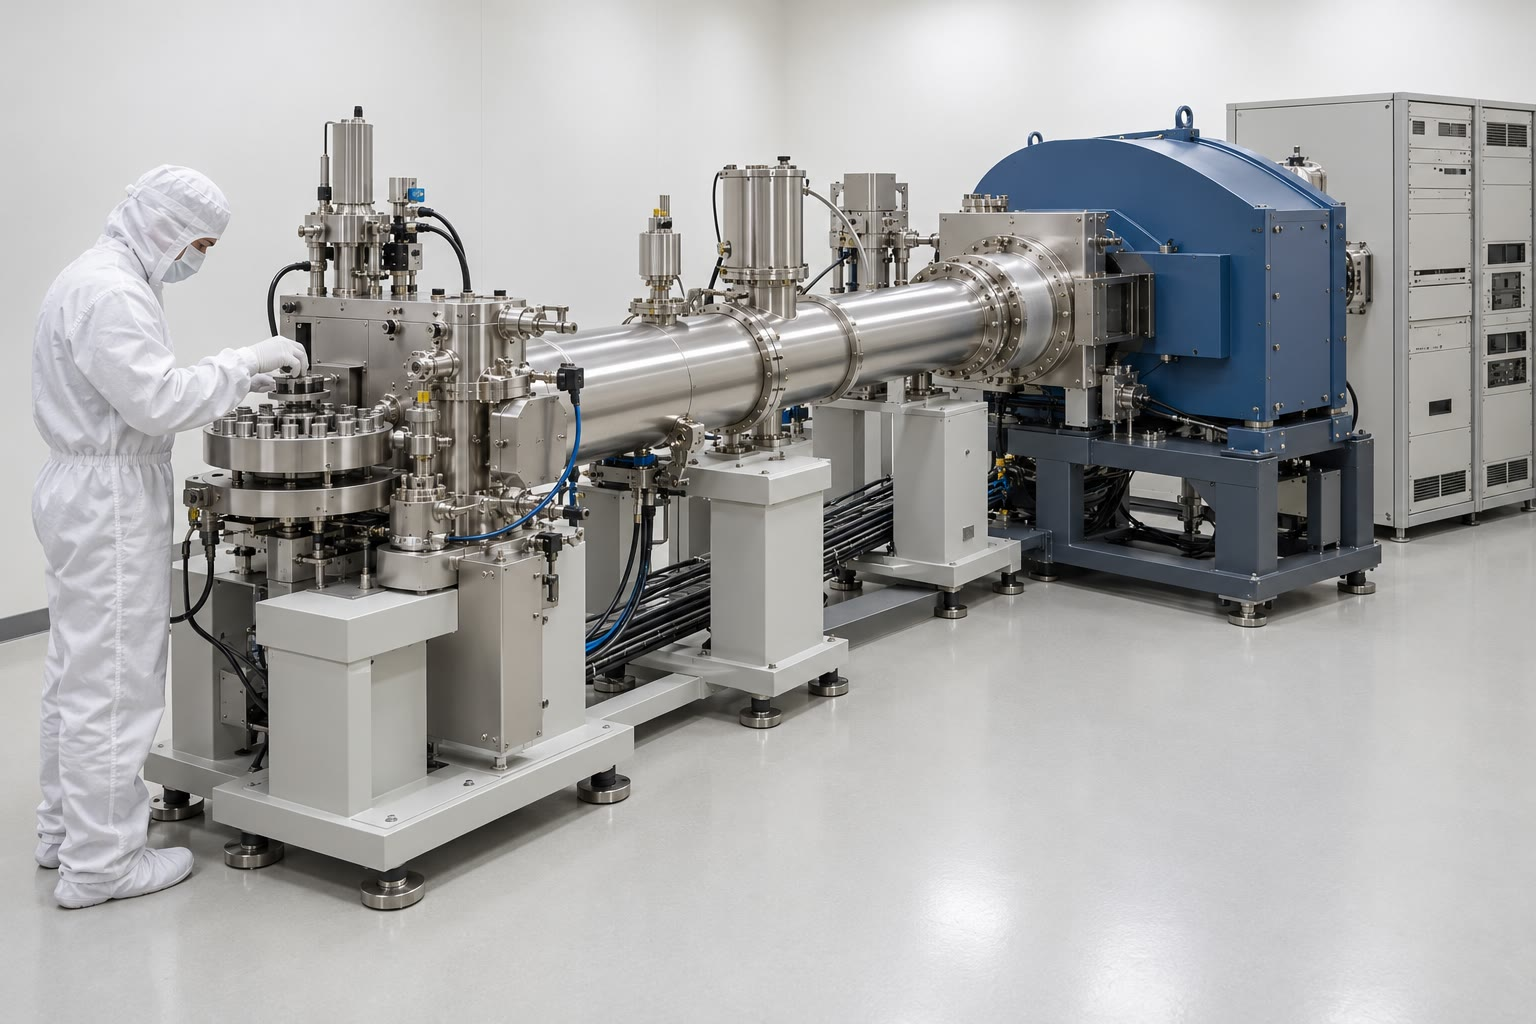
\includegraphics[width=\linewidth]{images/book5/ai/b3-mass-spec-lab.jpg}

{\scriptsize Un spectromètre de masse dans un laboratoire propre~: le plateau porte-échantillons à
gauche, le tube de vol et l'électroaimant (illustration générée
par IA).}
\end{minipage}
\end{inthelab}

\section{Datation argon--argon}\label{sec:b3:advanced-geochronology:arar}

La méthode potassium--argon du volume de première année mesure le potassium et
l'argon dans deux aliquotes séparées d'un minéral. La méthode argon--argon
ne mesure que l'argon, dans une seule aliquote, sous forme de rapports isotopiques. L'échantillon est
irradié par des neutrons rapides au cœur d'un réacteur nucléaire, où la
réaction $^{39}\mathrm{K}(n,p)^{39}\mathrm{Ar}$ transforme une fraction fixe de son
potassium-39 en argon-39, indicateur du potassium. Un minéral d'âge connu, le
moniteur, est irradié à côté.
% ledger: nmgrl:arar, amherst:arar

\begin{definition}[Datation argon--argon, facteur J, spectre d'âges, âge plateau]
\label{def:b3:advanced-geochronology:arar}
\emph{Datation $^{40}\mathrm{Ar}/^{39}\mathrm{Ar}$}\index{Datation $^{40}\mathrm{Ar}/^{39}\mathrm{Ar}$}
date un minéral porteur de potassium par le rapport $R =
{}^{40}\mathrm{Ar}^*/{}^{39}\mathrm{Ar}_{\mathrm K}$ de son argon-40 radiogénique
à l'argon-39 formé à partir de son potassium par irradiation neutronique. Le
\emph{facteur J}\index{facteur J} d'une irradiation est $J = (e^{\lambda
t_m} - 1)/R_m$, déterminé à partir d'un moniteur d'âge connu $t_m$ et d'un rapport mesuré
$R_m$, avec $\lambda$ la constante de désintégration totale du potassium-40. Lorsque
l'échantillon est dégazé par paliers de température croissante, son \emph{spectre
d'âges}\index{spectre d'âges} porte l'âge de chaque palier en fonction de la
fraction cumulée d'argon-39 libérée. Un \emph{âge
plateau}\index{âge plateau} est la moyenne pondérée de l'âge de paliers consécutifs qui
s'accordent dans leurs incertitudes et libèrent une grande part de l'argon-39.
\end{definition}

\begin{theorem}[L'âge argon--argon]\label{thm:b3:advanced-geochronology:arar}
Un échantillon irradié avec un moniteur a l'âge
\[
t = \frac1\lambda\ln(1 + JR).
\]
\end{theorem}

\begin{proof}
L'argon radiogénique vaut $^{40}\mathrm{Ar}^* = (\lambda_e/\lambda)\,
{}^{40}\mathrm{K}\,(e^{\lambda t} - 1)$, d'après la désintégration à embranchement du volume de
première année. L'argon-39 formé vaut $^{39}\mathrm{Ar}_{\mathrm K} =
{}^{39}\mathrm{K}\,\Phi$, où $\Phi$ rassemble la dose de neutrons et la
section efficace de la réaction. Donc $R = (e^{\lambda t} - 1)/J$ avec $J =
\lambda\,\Phi\,{}^{39}\mathrm{K}/(\lambda_e\,{}^{40}\mathrm{K})$. Le rapport
$^{40}\mathrm{K}/^{39}\mathrm{K}$ est le même dans tout le potassium, et $\Phi$ le
même pour deux échantillons irradiés côte à côte, donc $J$ est le même pour l'échantillon et le
moniteur~; l'âge et le rapport du moniteur le donnent, et l'inversion de $R$ donne
$t$.
\end{proof}

Les constantes sont celles de la méthode potassium--argon, $\lambda =
\qty{5.543e-10}{an^{-1}}$. Un moniteur courant est une sanidine d'un tuf volcanique
daté à \qty{28.201}{\Ma}~; un rapport du moniteur $R_m = 1.3129$ donne $J =
0.01200$. L'argon atmosphérique, avec $^{40}\mathrm{Ar}/^{36}\mathrm{Ar} = 295.5$,
est retranché à l'aide de l'argon-36 mesuré à chaque palier, et l'argon formé par les
neutrons à partir du calcium et du potassium lui-même est corrigé grâce à des sels
irradiés dans le même conditionnement.
% ledger: schaen20:monitors, amherst:constants, nmgrl:arar

La chauffe par paliers est la force de la méthode. L'échantillon est chauffé dans un four
ou par laser, par paliers de température croissante, et chaque palier donne un âge.
Si le minéral est resté clos depuis son refroidissement, tous les paliers concordent~: le spectre est
plat. S'il a perdu de l'argon par la bordure de ses grains, les premiers paliers, qui
proviennent de la bordure, sont plus jeunes, et les âges montent en escalier vers un
plateau donné par les cœurs. Les critères recommandés pour un plateau sont au
moins cinq paliers consécutifs portant plus de \qty{50}{\percent} de
l'argon-39, sans tendance entre eux~; les paliers à basse température d'un escalier
sont couramment interprétés comme une perte d'argon radiogénique. L'argon en excès, piégé dans un
fluide lors de la croissance du minéral, a l'effet inverse~: il rend certains paliers trop vieux,
souvent le premier et le dernier, dans un spectre en selle. La somme de tous les
paliers, l'âge du gaz total, est ce qu'aurait donné un âge potassium--argon~: une
moyenne qui masque l'histoire.
% ledger: schaen20:plateau, nmgrl:arar

\begin{omfigure}
\begin{tikzpicture}
\begin{groupplot}[group style={group size=2 by 1, horizontal sep=1.5cm},
  omrecord, height=0.38\linewidth, title style={font=\small},
  xlabel={$^{39}\mathrm{Ar}$ libéré cumulé (\unit{\percent})},
  tick label style={font=\scriptsize}, label style={font=\small}]
\nextgroupplot[title={(a) le spectre entier}, width=0.52\linewidth,
  ylabel={âge apparent (\unit{\Ma})}, xmin=0, xmax=100, ymin=130, ymax=320,
  xtick={0,20,40,60,80,100}, ytick={150,200,250,300}]
% computed in figdata/bachelor-3/arar_spectrum.py
\addplot[omDef, thick] table[x=cum, y=age] {figdata/out/bachelor-3-arar_spectrum-boxes.dat};
\node[font=\scriptsize, anchor=west] at (axis cs:12,180) {perte d'argon};
\node[font=\scriptsize, anchor=north, red!70!black] at (axis cs:59,290) {plateau};
\nextgroupplot[title={(b) le plateau, agrandi}, width=0.44\linewidth,
  xmin=15, xmax=100, ymin=290, ymax=300, xtick={20,40,60,80,100},
  ytick={290,292,294,296,298,300}]
\addplot[name path=hi, draw=none, forget plot] table[x=cum, y=hi] {figdata/out/bachelor-3-arar_spectrum-boxes.dat};
\addplot[name path=lo, draw=none, forget plot] table[x=cum, y=lo] {figdata/out/bachelor-3-arar_spectrum-boxes.dat};
\addplot[omDef!25, forget plot] fill between[of=hi and lo];
\addplot[omDef, thick] table[x=cum, y=age] {figdata/out/bachelor-3-arar_spectrum-boxes.dat};
\draw[red!70!black, thick] (axis cs:18,296.1) -- (axis cs:100,296.1);
\node[font=\scriptsize, anchor=south, red!70!black] at (axis cs:59,290.3) {âge plateau \qty[separate-uncertainty=true]{296.1 \pm 0.8}{\Ma}};
\end{groupplot}
\end{tikzpicture}

\par\smallskip{\small Le \omterm{def:b3:advanced-geochronology:arar}{spectre d'âges} fictif d'une biotite du granite de
la première figure~: chaque palier est tracé à son âge, sa largeur représentant la part de
l'argon-39 qu'il a libéré. (a) Trois paliers à basse température montent en escalier vers un
plateau. (b) Les sept paliers du plateau, qui portent \qty{82}{\percent} de
l'argon-39, avec leurs intervalles à deux écarts-types (en grisé) et l'\omterm{def:b3:advanced-geochronology:arar}{âge plateau}
plateau (en rouge).}\label{fig:b3:advanced-geochronology:spectrum}
\end{omfigure}

\section{Âges modèles du néodyme}\label{sec:b3:advanced-geochronology:model-age}

Lorsqu'un liquide est extrait du manteau pour former la croûte continentale, le samarium,
plus compatible, reste davantage dans le résidu que le néodyme~: la nouvelle croûte a un
$^{147}\mathrm{Sm}/^{144}\mathrm{Nd}$ plus faible que sa source, d'environ 0.13 pour la plupart
des roches crustales, contre 0.1966 pour le réservoir chondritique. Son
$^{143}\mathrm{Nd}/^{144}\mathrm{Nd}$ croît alors plus lentement. Une fois formée, une
roche crustale tend à conserver son rapport samarium--néodyme, malgré l'érosion,
la sédimentation et même la refusion, si bien que son néodyme garde la trace du moment où il a quitté le
manteau.
% ledger: white08:model-age, white:chur

\begin{definition}[Âge modèle]\label{def:b3:advanced-geochronology:model-age}
L'\emph{âge modèle}\index{age modele@âge modèle} d'une roche dans un système isotopique est le
instant où son rapport, extrapolé vers le passé avec son rapport parent--fils actuel,
égal à celui d'un réservoir modèle. Pour le néodyme, $T_{\mathrm{CHUR}}$
utilise le réservoir uniforme chondritique et $T_{\mathrm{DM}}$ le manteau
appauvri.
\end{definition}

\begin{theorem}[Âge modèle]\label{thm:b3:advanced-geochronology:model-age}
Un échantillon de rapports actuels $I_s = {}^{143}\mathrm{Nd}/^{144}\mathrm{Nd}$ et
$R_s = {}^{147}\mathrm{Sm}/^{144}\mathrm{Nd}$, comparé à un réservoir de
rapports actuels $I_m$ et $R_m$, admet l'\omterm{def:b3:advanced-geochronology:model-age}{âge modèle}
\[
T = \frac1\lambda\ln\left(1 + \frac{I_s - I_m}{R_s - R_m}\right),
\qquad \lambda = \lambda_{147}.
\]
\end{theorem}

\begin{proof}
Un système clos avait, un temps $T$ plus tôt, le rapport $I - R(e^{\lambda T} - 1)$~:
l'équation de l'isochrone lue à rebours. En égalant cette expression pour l'échantillon et le
réservoir donne $I_s - I_m = (R_s - R_m)(e^{\lambda T} - 1)$.
\end{proof}

Avec $\lambda_{147} = \qty{6.524e-12}{an^{-1}}$, les réservoirs sont le
chondritique, 0.512638 et 0.1966 aujourd'hui, et le manteau
appauvri, 0.51315 aujourd'hui, soit environ $\varepsilon_{\mathrm{Nd}} = +10$, ce que donne une évolution close
à partir de valeurs chondritiques depuis \qty{4.55}{\Ga} donne le rapport
$^{147}\mathrm{Sm}/^{144}\mathrm{Nd} = 0.2137$. Un granite fictif, avec
$I_s = 0.511900$ et $R_s = 0.1100$ présente $\varepsilon_{\mathrm{Nd}} = -14.4$
aujourd'hui, $T_{\mathrm{CHUR}} = \qty{1.30}{\Ga}$ et $T_{\mathrm{DM}} =
\qty{1.84}{\Ga}$. La figure ci-dessous donne les deux. L'âge du manteau appauvri est le
meilleure estimation, car la croûte est extraite d'un manteau déjà
appauvri~; c'est l'âge moyen auquel le néodyme de l'échantillon a quitté le
manteau, son âge de résidence crustale. Deux réserves en limitent la portée~: la croûte ne doit pas
avoir modifié son rapport samarium--néodyme depuis, et une roche formée par mélange
de croûte ancienne et de liquides issus d'un manteau récent a un \omterm{def:b3:advanced-geochronology:model-age}{âge modèle} intermédiaire dépourvu de sens.
% ledger: villa20:sm147, white:chur, white08:model-age

\begin{omfigure}
\begin{tikzpicture}
\begin{axis}[omrecord, width=0.72\linewidth, height=0.38\linewidth,
  xlabel={temps avant le présent (\unit{\Ga})}, ylabel={$\varepsilon_{\mathrm{Nd}}$},
  xmin=0, xmax=2.5, ymin=-17, ymax=13, x dir=reverse,
  xtick={0,0.5,1,1.5,2,2.5}, xticklabels={0,0.5,1,1.5,2,2.5},
  tick label style={font=\scriptsize}, label style={font=\small},
  legend style={font=\scriptsize, at={(0.5,1.03)}, anchor=south, legend columns=3, legend cell align=left}]
% computed in figdata/bachelor-3/model_ages.py
\addplot[omDef, thick] table[x=t, y=eps_dm] {figdata/out/bachelor-3-model_ages-evolution.dat};
\addlegendentry{manteau appauvri}
\addplot[black, thick, densely dashed] coordinates {(0,0) (2.5,0)};
\addlegendentry{CHUR}
\addplot[red!70!black, thick] table[x=t, y=eps_sample] {figdata/out/bachelor-3-model_ages-evolution.dat};
\addlegendentry{granite}
\draw[densely dotted] (axis cs:1.30,0) -- (axis cs:1.30,-17) node[above right, font=\scriptsize, rotate=90] {$T_{\mathrm{CHUR}}$};
\draw[densely dotted] (axis cs:1.84,5.4) -- (axis cs:1.84,-17) node[above right, font=\scriptsize, rotate=90] {$T_{\mathrm{DM}}$};
\end{axis}
\end{tikzpicture}

\par\smallskip{\small $\varepsilon_{\mathrm{Nd}}$ d'un granite fictif reporté dans le temps
avec son propre rapport samarium--néodyme (rouge). Il rejoint le
réservoir chondritique à $T_{\mathrm{CHUR}} = \qty{1.30}{\Ga}$ et le
manteau appauvri (bleu) à $T_{\mathrm{DM}} = \qty{1.84}{\Ga}$.}\label{fig:b3:advanced-geochronology:model-age}
\end{omfigure}

\section{Datation par traces de fission et hélium}\label{sec:b3:advanced-geochronology:low-t}

L'uranium-238 se désintègre aussi, très rarement, par fission spontanée~: le noyau
se scinde en deux fragments qui s'éloignent et laissent une trace de dommages dans le
cristal, large d'environ \qty{9}{nm} et longue d'environ \qty{23}{\micro\metre} dans
l'apatite. Attaquées à l'acide, les traces deviennent visibles au microscope.
Elles guérissent lorsque le cristal est chauffé, entre environ 20 et \qty{350}{\celsius}
selon le minéral~; dans l'apatite, elles se raccourcissent dans la zone de recuit partiel,
d'environ 60 à \qty{120}{\celsius}, et disparaissent au-dessus.
% ledger: kohn24:ft, sueoka19:closure

\begin{definition}[Datation par traces de fission, recuit des traces]\label{def:b3:advanced-geochronology:fission-track}
La \emph{datation par traces de fission}\index{datation par traces de fission} date un minéral par
la densité des traces laissées en lui par la fission spontanée de
l'uranium-238, rapportée à sa teneur en uranium. Le \emph{recuit des
traces}\index{recuit des traces} est le raccourcissement et la disparition des
traces par la réparation du cristal lorsqu'il est chauffé.
\end{definition}

\begin{theorem}[L'âge par traces de fission]\label{thm:b3:advanced-geochronology:fission-track}
Avec $\lambda_f$ la constante de désintégration de la fission spontanée et $\lambda =
\lambda_{238}$ la constante totale, un cristal comportant $N_s$ fissions spontanées par unité
de volume et $N$ atomes d'uranium-238 a pour âge
\[
t = \frac1\lambda\ln\left(1 + \frac{\lambda}{\lambda_f}\,\frac{N_s}{N}\right).
\]
En laboratoire, l'uranium est mesuré en provoquant la fission de
l'uranium-235 par des neutrons thermiques, et l'âge devient
\[
t = \frac1\lambda\ln\left(1 + \lambda\,\zeta\,g\,\rho_d\,\frac{\rho_s}{\rho_i}\right),
\]
avec $\rho_s$ et $\rho_i$ les densités de traces spontanées et induites,
$\rho_d$ la densité de traces d'un verre dosimètre, $g = 0.5$ un facteur
géométrique et $\zeta$ une constante d'étalonnage établie sur des étalons d'âge connu.
\end{theorem}

\begin{proof}
L'uranium-238 s'est désintégré $N(e^{\lambda t} - 1)$ fois, et la fraction
$\lambda_f/\lambda$ de ces désintégrations sont des fissions~: $N_s =
(\lambda_f/\lambda)N(e^{\lambda t} - 1)$, ce qui s'inverse en la première forme.
Les densités de traces sont proportionnelles à $N_s$ et au nombre de fissions
induites, $N\,\sigma\,\Phi/137.8$, où $\sigma$ est la section efficace de
fission de l'uranium-235 et $\Phi$ la fluence neutronique, elle-même
proportionnelle à $\rho_d$. Le rapport $\rho_s/\rho_i$ vaut alors $N_s/N$ multiplié
par un produit de constantes, et $\lambda_f$, $\sigma$, $137.8$ ainsi que l'efficacité
d'attaque et de comptage sont regroupés avec $g$ dans $\zeta$.
\end{proof}

La constante de désintégration par fission n'est connue qu'à environ \qty{10}{\percent} près,
entre \num{7.9e-17} et \qty{8.7e-17}{an^{-1}}, raison pour laquelle la plupart des
laboratoires préfèrent l'étalonnage par $\zeta$. La longueur des traces garde
la mémoire du parcours thermique. Une roche refroidie rapidement à travers la
zone de recuit partiel possède de longues traces de longueurs presque égales~; une
roche qui y est restée longtemps présente des traces plus courtes, de longueurs très dispersées, et
l'âge par traces de fission est alors un âge mixte, qui ne correspond pas au moment
d'un passage à une seule température.
% ledger: kohn24:ft

\begin{omfigure}
\begin{tikzpicture}[scale=0.85]
% (a) an etched apatite grain with tracks
\draw[thick, fill=omLithLime!15] (0,0) -- (3.2,0) -- (3.8,1.0) -- (3.2,2.0) -- (0,2.0) -- (-0.6,1.0) -- cycle;
\foreach \x/\y/\a in {0.4/0.5/30, 1.2/1.3/-20, 2.0/0.6/75, 2.6/1.4/10, 0.9/1.6/110, 1.7/0.9/150, 2.9/0.8/50}
  {\draw[very thick, black] (\x,\y) -- ++(\a:0.45);}
\node[font=\small] at (1.6,-0.4) {(a) traces de fission attaquées dans l'apatite};
% (b) alpha ejection from a grain
\begin{scope}[xshift=6cm]
\draw[thick, fill=omLithLime!15] (0,0) rectangle (3.4,2.0);
\draw[dashed] (0.35,0.35) rectangle (3.05,1.65);
\fill[black] (0.2,1.0) circle (1.5pt) node[below right, font=\scriptsize] {U};
\draw[->, red!70!black, thick] (0.2,1.0) -- ++(160:0.7) node[left, font=\scriptsize] {He perdu};
\fill[black] (1.7,1.0) circle (1.5pt);
\draw[->, red!70!black, thick] (1.7,1.0) -- ++(40:0.5);
\node[font=\scriptsize, align=center] at (1.7,0.55) {He conservé};
\draw[<->] (3.05,1.8) -- (3.4,1.8) node[right, font=\scriptsize] {\qty{20}{\micro\metre}};
\node[font=\small] at (1.7,-0.4) {(b) émission alpha};
\end{scope}
\end{tikzpicture}

\par\smallskip{\small Schéma. (a) Traces de fission spontanée, révélées par
attaque sur un grain d'apatite poli, comptées par unité de surface. (b) Une particule
alpha parcourt environ \qty{20}{\micro\metre}~: celles émises à moins de cette
distance de la surface (à l'extérieur du trait pointillé) peuvent quitter le grain, si bien
qu'un petit grain conserve moins de son hélium.}\label{fig:b3:advanced-geochronology:low-t}
\end{omfigure}
% ledger: zeigler23:ejection

Chaque désintégration alpha émet un noyau d'hélium-4. L'uranium, le thorium et leurs
chaînes accumulent l'hélium dans un cristal, qui ne le retient que lorsqu'il est froid.

\begin{definition}[Datation (U--Th)/He, zone de rétention partielle]\label{def:b3:advanced-geochronology:uthhe}
La \emph{datation (U--Th)/He}\index{datation (U--Th)/He} date un
minéral par l'hélium-4 accumulé à partir des désintégrations alpha de l'uranium, du thorium
et de leurs descendants, rapporté à sa teneur en uranium et en thorium. La \emph{zone de
rétention partielle}\index{zone de rétention partielle} est l'intervalle de température
dans lequel l'hélium produit est en partie conservé et en partie perdu par diffusion.
\end{definition}

\begin{theorem}[Accumulation de l'hélium]\label{thm:b3:advanced-geochronology:helium}
Un cristal fermé à l'hélium pendant un temps $t$ contient
\[
\mathrm{He} = 8\,{}^{238}\mathrm U\,(e^{\lambda_{238}t} - 1)
+ 7\,{}^{235}\mathrm U\,(e^{\lambda_{235}t} - 1)
+ 6\,{}^{232}\mathrm{Th}\,(e^{\lambda_{232}t} - 1),
\]
en atomes, les parents étant mesurés aujourd'hui~; le samarium-147 ajoute un petit terme.
\end{theorem}

\begin{proof}
Chaque chaîne perd sa différence de masse en particules alpha, quatre unités de masse chacune~:
$(238 - 206)/4 = 8$, $(235 - 207)/4 = 7$, $(232 - 208)/4 = 6$, tandis que les désintégrations bêta
ne modifient pas le nombre de masse. Chaque chaîne est à l'équilibre séculaire,
de sorte que chaque désintégration du parent est suivie de toute sa chaîne, et le nombre de
désintégrations de chaque parent est celui de l'équation d'âge.
\end{proof}

Pour un cristal jeune, $e^{\lambda t} - 1 \approx \lambda t$ et l'âge découle
d'une simple division. Une particule alpha parcourt environ
\qty{20}{\micro\metre} avant de s'arrêter, si bien qu'un cristal perd l'hélium formé
près de sa surface~; l'âge mesuré est divisé par la fraction retenue $F_T$,
qui est plus faible pour les petits grains ($F_T = 0.70$ signifie que \qty{30}{\percent}
perdus). L'apatite se ferme à l'hélium vers 50 à \qty{80}{\celsius}, le zircon vers
160 à \qty{200}{\celsius}~: avec les traces de fission de l'apatite, vers 90 à
\qty{120}{\celsius}, les chronomètres basse température datent les derniers
kilomètres de la remontée d'une roche vers la surface, comme
l'a fait le \cref{ch:b3:orogenic-wedges}.
% ledger: zeigler23:ejection, sueoka19:closure, iaea:isotopes

\section{Nucléides cosmogéniques}\label{sec:b3:advanced-geochronology:cosmogenic}

Les rayons cosmiques qui frappent l'atmosphère produisent des gerbes de particules secondaires. Les
neutrons rapides qui atteignent le sol brisent les noyaux des minéraux des premiers
mètres de roche, par spallation~: l'oxygène du quartz devient du béryllium-10, le silicium
devient de l'aluminium-26. Les muons forment certains nucléides plus profondément et dominent au-dessous d'environ
\qty{3}{m}.
% ledger: zech04:exposure, portenga:method

\begin{definition}[Nucléide cosmogénique, âge d'exposition, taux de production]
\label{def:b3:advanced-geochronology:cosmogenic}
Un \emph{nucléide cosmogénique}\index{nucléide cosmogénique} est un nucléide formé
dans un minéral à la surface ou près de celle-ci par les particules secondaires des rayons cosmiques. Son
\emph{taux de production}\index{taux de production (cosmogénique)} $P$ est le nombre
d'atomes formés par unité de masse de minéral et par an. L'\emph{âge
d'exposition}\index{age@âge d'exposition} d'une surface est le temps écoulé depuis sa première exposition
aux rayons cosmiques, déduit de la concentration d'un nucléide cosmogénique.
\end{definition}

Le \omterm{def:b3:advanced-geochronology:cosmogenic}{taux de production} décroît avec la profondeur selon $P_0e^{-\rho z/\Lambda}$, où
la longueur d'atténuation vaut $\Lambda = \qty{160}{g.cm^{-2}}$, soit environ
\qty{60}{cm} de granite de masse volumique \qty{2.7}{g.cm^{-3}}. À la surface, il
croît avec l'altitude, car moins d'air protège la roche, et avec
la latitude géomagnétique, car le champ dévie moins de particules près des
pôles. Les taux sont donnés pour une référence au niveau de la mer et à haute latitude, puis
adaptés à chaque site~: un étalonnage donne $P_0 = \qty{4.96}{atomes.g^{-1}.an^{-1}}$
de béryllium-10 dans le quartz pour cette référence. Le béryllium-10 a une demi-vie de
\qty{1.388}{Ma}, $\lambda = \qty{4.994e-7}{an^{-1}}$.
% ledger: balco08:params, zech04:exposure, lugaro:slr-table

\begin{theorem}[Exposition avec désintégration et érosion]\label{thm:b3:advanced-geochronology:exposure}
Une surface abaissée à la vitesse constante $\varepsilon$, exposée pendant un temps $t$
sans nucléide hérité, porte à sa surface la concentration
\[
N(t) = \frac{P_0}{\mu}\bigl(1 - e^{-\mu t}\bigr), \qquad
\mu = \lambda + \frac{\rho\varepsilon}{\Lambda}.
\]
Sans érosion, $N = (P_0/\lambda)(1 - e^{-\lambda t})$~; après un long temps,
$N = P_0/\mu$, et sans désintégration on retrouve la formule $P_0\Lambda/(\rho\varepsilon)$
du volume de première année.
\end{theorem}

\begin{proof}
Suivons le grain qui se trouve aujourd'hui à la surface. Il y a un temps $s$, il se trouvait à la
profondeur $\varepsilon s$, où il gagnait des atomes au taux $P_0e^{-\rho\varepsilon
s/\Lambda}$~; de ces atomes, la fraction $e^{-\lambda s}$ subsiste aujourd'hui. En sommant
sur toute l'exposition,
\[
N = \int_0^t P_0e^{-\rho\varepsilon s/\Lambda}e^{-\lambda s}\,\mathrm ds
= \frac{P_0}{\mu}\bigl(1 - e^{-\mu t}\bigr).
\]
Les cas limites s'obtiennent en posant $\varepsilon = 0$, en faisant tendre $t \to \infty$, et
ensuite $\lambda = 0$.
\end{proof}

Sans érosion, la concentration sature à $P_0/\lambda$ au bout de quelques
demi-vies~: une surface atteint \qty{90}{\percent} de cette valeur après $\ln 10/\lambda
= \qty{4.6}{Ma}$, et au-delà elle ne peut plus être datée. Avec l'érosion,
l'état stationnaire est atteint plus tôt, au bout de quelques fois $1/\mu$, et sa
concentration donne $\varepsilon$~; le taux est moyenné sur le temps
$\Lambda/(\rho\varepsilon)$ mis par le grain pour remonter à travers une
longueur d'atténuation, soit quelques dizaines de milliers d'années aux taux de quelques
dizaines de mètres par million d'années. Les affleurements de substratum rocheux s'érodent à quelques mètres
à quelques dizaines de mètres par million d'années~; les bassins fluviaux, mesurés à partir des
sables de leurs rivières, plus rapidement.
% ledger: portenga:rates, portenga:method

Deux nucléides de demi-vies différentes datent l'enfouissement. Le béryllium-10 et
l'aluminium-26 se forment ensemble dans le quartz selon un rapport fixe~; lorsqu'un grain est
enfoui profondément dans une grotte ou sous un épais sédiment, la production cesse, et
l'aluminium-26, qui se désintègre plus vite, prend du retard~: le rapport des deux
décroît avec le temps et date l'enfouissement.

\section{Statistique d'un âge}\label{sec:b3:advanced-geochronology:statistics}

Un âge s'accompagne de son incertitude, et un ensemble d'âges de la question
de savoir s'ils concordent. Soient $n$ mesures $x_i$ d'une même grandeur, d'écarts types
$\sigma_i$. Leur moyenne pondérée vaut $\bar x = \sum w_ix_i/W$, avec
$w_i = 1/\sigma_i^2$ et $W = \sum w_i$, et son écart type vaut
$1/\sqrt W$.

\begin{definition}[Moyenne des carrés des écarts pondérés]\label{def:b3:advanced-geochronology:mswd}
La \emph{moyenne des carrés des écarts pondérés}\index{moyenne des carrés des écarts pondérés}
(MSWD) de $n$ mesures par rapport à un modèle ajusté à $p$ paramètres ajustables
est
\[
\mathrm{MSWD} = \frac{1}{n - p}\sum_i \frac{(x_i - \hat x_i)^2}{\sigma_i^2},
\]
où $\hat x_i$ est la valeur du modèle~: $p = 1$ pour une moyenne pondérée, $p = 2$ pour
une droite comme une isochrone ou une \omterm{def:b3:advanced-geochronology:concordia}{discordia}.
\end{definition}

\begin{proposition}[La MSWD a pour espérance un]\label{prop:b3:advanced-geochronology:mswd}
Si les $x_i$ sont indépendants, gaussiens, de moyenne $\mu$ et d'écarts types
$\sigma_i$, la MSWD par rapport à leur moyenne pondérée a pour espérance 1.
\end{proposition}

\begin{proof}
En développant $x_i - \mu = (x_i - \bar x) + (\bar x - \mu)$ et en utilisant $\sum
w_i(x_i - \bar x) = 0$,
\[
\sum w_i(x_i - \mu)^2 = \sum w_i(x_i - \bar x)^2 + W(\bar x - \mu)^2.
\]
À gauche, chaque terme a pour espérance 1, donc la somme a pour espérance $n$.
À droite, $\bar x$ a pour variance $1/W$, donc le dernier terme a pour espérance 1.
D'où $\sum w_i(x_i - \bar x)^2$ a pour espérance $n - 1$.
\end{proof}

La MSWD se disperse davantage autour de 1 lorsque le nombre de degrés de liberté est
faible, $f = n - p$~: sa limite supérieure à \qty{95}{\percent} vaut environ $1 +
2\sqrt{2/f}$, 2.63 pour $f = 3$ et 2.15 pour $f = 6$. Au-delà de la limite, les
mesures se dispersent davantage que ne le permettent leurs incertitudes~: les
échantillons n'ont pas tous le même âge, ou que le système a été perturbé. Très
en dessous de 1, les incertitudes ont été surestimées.
% ledger: schaen20:mswd

\begin{method}[Ajustement d'une isochrone avec erreurs sur les deux axes]\label{met:b3:advanced-geochronology:york}
Lorsque les deux coordonnées portent des erreurs $\sigma_{x,i}$, $\sigma_{y,i}$, corrélées
avec le coefficient $r_i$, comme pour les données uranium--plomb et isochrones~:
\begin{enumerate}
\item partir de la pente $b$ de la droite des moindres carrés ordinaires~;
\item affecter à chaque point le poids $W_i = 1/(\sigma_{y,i}^2 + b^2\sigma_{x,i}^2 -
2br_i\sigma_{x,i}\sigma_{y,i})$, l'inverse de la variance de sa distance à la
droite mesurée selon $y$~;
\item ajuster la droite pondérée avec ces poids, ce qui donne un nouveau $b$, et
revenir à l'étape 2 jusqu'à ce que $b$ ne change plus~;
\item calculer la MSWD avec les poids $W_i$ et $n - 2$ degrés de liberté,
ainsi que l'incertitude de la pente et de l'ordonnée à l'origine à partir des poids finaux.
\end{enumerate}
Si $\sigma_{x,i} = 0$, les poids ne dépendent pas de $b$, et la méthode
se réduit aux moindres carrés pondérés de $y$ sur $x$ utilisés dans le problème.
\end{method}

L'incertitude d'une constante de désintégration est la même pour tous les âges d'un système~:
elle n'intervient pas lorsqu'on compare des âges d'un même système, mais doit être
ajoutée lorsque l'on compare des âges issus de deux systèmes. La constante de
désintégration du samarium-147, par exemple, est connue à environ \qty{0.4}{\percent} près~;
celles du potassium-40, dont la désintégration est lente et à embranchement, limitent la précision des âges argon.
% ledger: villa20:sm147, nmgrl:arar


\section{Exercices}

\begin{exercise}[$\star$]\label{exo:b3:advanced-geochronology:1}
Un zircon possède $^{206}\mathrm{Pb}^*/^{238}\mathrm{U} = 0.04500$ et
$^{207}\mathrm{Pb}^*/^{235}\mathrm{U} = 0.3300$. Calculer ses deux âges
uranium--plomb. Est-il concordant~? De quel côté de la \omterm{def:b3:advanced-geochronology:concordia}{concordia}
se place-t-il~? 
\end{exercise}
% ledger: amherst:constants

\begin{exercise}[$\star$]\label{exo:b3:advanced-geochronology:2}
Un moniteur de \qty{28.201}{\Ma} donne $R_m = 1.3129$. Calculer $J$ avec $\lambda
= \qty{5.543e-10}{an^{-1}}$, puis l'âge d'un échantillon de la même irradiation
avec $R = 10.000$ (utiliser $J = 0.01200$).
\end{exercise}
% ledger: schaen20:monitors

\begin{exercise}[$\star$]\label{exo:b3:advanced-geochronology:3}
Une argilite possède $^{143}\mathrm{Nd}/^{144}\mathrm{Nd} = 0.51180$ et
$^{147}\mathrm{Sm}/^{144}\mathrm{Nd} = 0.1200$. Calculer son $T_{\mathrm{CHUR}}$
et son $T_{\mathrm{DM}}$ avec les valeurs du chapitre.
\end{exercise}
% ledger: villa20:sm147, white:chur, white08:model-age

\begin{exercise}[$\star$]\label{exo:b3:advanced-geochronology:4}
Un bloc de quartz posé sur une moraine du site de référence contient \num{2.0e5}
atomes de béryllium-10 par gramme. En supposant l'absence d'érosion et d'héritage,
calculer son \omterm{def:b3:advanced-geochronology:cosmogenic}{âge d'exposition} sans puis avec décroissance, avec $P_0 =
\qty{4.96}{atomes.g^{-1}.an^{-1}}$.
\end{exercise}
% ledger: balco08:params, lugaro:slr-table

\begin{exercise}[$\star\star$]\label{exo:b3:advanced-geochronology:5}
Montrer qu'au voisinage de l'origine la \omterm{def:b3:advanced-geochronology:concordia}{concordia} est une droite de pente
$\lambda_{238}/\lambda_{235}$, et la calculer. Expliquer pourquoi la \omterm{def:b3:advanced-geochronology:concordia}{discordia} des
cristaux ayant perdu du plomb très récemment passe par l'origine, et
ce que mesure l'âge plomb--plomb de tels cristaux.
\end{exercise}

\begin{exercise}[$\star\star$]\label{exo:b3:advanced-geochronology:6}
Quatre âges par paliers d'un plateau valent $296.4 \pm 0.8$, $295.1 \pm 1.0$, $297.0 \pm
0.9$ et \qty[separate-uncertainty=true]{295.8 \pm 0.7}{\Ma} ($1\sigma$). Calculer leur moyenne pondérée,
son écart type et la MSWD. Sont-ils compatibles~?
\end{exercise}
% ledger: schaen20:mswd

\begin{exercise}[$\star\star$]\label{exo:b3:advanced-geochronology:7}
Une apatite possède $\rho_s = \qty{1.20e6}{cm^{-2}}$ et $\rho_i =
\qty{2.40e6}{cm^{-2}}$, avec $\rho_d = \qty{1.10e6}{cm^{-2}}$, $g = 0.5$ et un
étalonnage en laboratoire $\zeta = \qty{350}{an.cm^2}$. Calculer son âge par traces
de fission. Quel événement date-t-il~?
\end{exercise}
% ledger: kohn24:ft, sueoka19:closure

\begin{exercise}[$\star\star$]\label{exo:b3:advanced-geochronology:8}
Une apatite contient \qty{20}{ppm} d'uranium (\qty{99.2742}{\percent}
d'uranium-238, \qty{0.7204}{\percent} d'uranium-235 en nombre d'atomes), \qty{40}{ppm}
de thorium-232 (demi-vie \qty{1.40e10}{an}) et \qty{1.0}{nmol.g^{-1}} d'hélium.
Calculer son âge (U--Th)/He avec l'approximation linéaire, puis l'âge
corrigé de l'éjection alpha avec $F_T = 0.75$.
\end{exercise}
% ledger: iaea:isotopes, zeigler23:ejection

\begin{exercise}[$\star\star$]\label{exo:b3:advanced-geochronology:9}
Pour le béryllium-10 sur le site de référence, calculer la concentration à saturation
sans érosion et le temps nécessaire pour atteindre \qty{90}{\percent} de celle-ci. Calculer la
concentration stationnaire d'une surface s'érodant à \qty{10}{m.Ma^{-1}} (granite,
\qty{2.7}{g.cm^{-3}}, $\Lambda = \qty{160}{g.cm^{-2}}$).
\end{exercise}
% ledger: balco08:params, zech04:exposure, lugaro:slr-table

\begin{exercise}[$\star\star\star$]\label{exo:b3:advanced-geochronology:10}
Deux mesures $x_1 \pm \sigma_1$ et $x_2 \pm \sigma_2$ d'un même âge sont
combinées. Montrer que leur MSWD par rapport à la moyenne pondérée vaut
$(x_1 - x_2)^2/(\sigma_1^2 + \sigma_2^2)$, et démontrer directement que son
espérance vaut 1 lorsque les deux mesurent le même âge.
\end{exercise}

\begin{exercise}[$\star\star\star$]\label{exo:b3:advanced-geochronology:11}
Un zircon de \qty{2700}{\Ma} a perdu du plomb à \qty{500}{\Ma} et présente aujourd'hui
$^{206}\mathrm{Pb}^*/^{238}\mathrm{U} = 0.300$. Quelle fraction de son plomb a-t-il
perdue~? Calculer son $^{207}\mathrm{Pb}^*/^{235}\mathrm{U}$, ses deux âges uranium--plomb
et, par itération, son âge plomb--plomb. Lequel des trois âges a-t-il un
sens~?
\end{exercise}

\begin{exercise}[$\star\star\star$]\label{exo:b3:advanced-geochronology:12}
Une surface de substratum sur le site de référence contient \num{1.0e6} atomes de
béryllium-10 par gramme. Calculer son \omterm{def:b3:advanced-geochronology:cosmogenic}{âge d'exposition} en supposant l'absence d'érosion, puis sa
vitesse d'érosion en supposant un état stationnaire. Montrer que chaque couple $(t, \varepsilon)$
compris entre ces deux limites correspond à la mesure, et indiquer quelle seconde
mesure permettrait de les départager.
\end{exercise}

\section{Problème~: Zircons du granite de Varden}

\begin{problem}[{Problème du week-end --- la cristallisation, le refroidissement et
le décapage d'un granite fictif, lus sur quatre horloges}]\label{pb:b3:advanced-geochronology:1}
Le granite des collines de Varden, région fictive de la série, a été décapé
avant le Trias, enfoui sous la couverture mésozoïque puis ramené à la
surface. Cinq de ses zircons donnent, avec des erreurs d'un écart type sur $y$
(prendre $x$ exact)~:
\begin{center}
\small
\begin{tabular}{|l|ccccc|}
\hline
zircon & Z1 & Z2 & Z3 & Z4 & Z5 \\
\hline
$x = {}^{207}\mathrm{Pb}^*/^{235}\mathrm U$ & 0.3467 & 0.3260 & 0.3027 & 0.2793 & 0.2535 \\
$y = {}^{206}\mathrm{Pb}^*/^{238}\mathrm U$ & 0.04794 & 0.04505 & 0.04207 & 0.03892 & 0.03553 \\
$\sigma_y$ & 0.00010 & 0.00009 & 0.00008 & 0.00008 & 0.00007 \\
\hline
\end{tabular}
\end{center}
Utiliser les constantes du chapitre. Toutes les analyses sont des données d'exercice.
% ledger: amherst:constants, schaen20:monitors, schaen20:plateau, schaen20:mswd, sueoka19:closure, balco08:params, lugaro:slr-table

\medskip\noindent\textbf{Partie I --- Les zircons.}
\begin{enumerate}
\item Calculer les deux âges uranium--plomb de chaque zircon. Sont-ils concordants~?
\item Pourquoi les âges diminuent-ils de Z1 à Z5, avec $t_{207} > t_{206}$ pour
chacun~?
\item Calculer les coordonnées de Tera--Wasserburg de Z1 et Z5.
\item Avec les poids $w_i = 1/\sigma_{y,i}^2$, calculer les moyennes pondérées
$\bar x$ et $\bar y$ ainsi que $S_{xx} = \sum w_i(x_i - \bar x)^2$.
\item Calculer la pente $b = \sum w_i(x_i - \bar x)(y_i - \bar y)/S_{xx}$ et
l'ordonnée à l'origine $a$ de la \omterm{def:b3:advanced-geochronology:concordia}{discordia}.
\item Comparer $b$ à la pente de la \omterm{def:b3:advanced-geochronology:concordia}{concordia} au voisinage de \qty{310}{\Ma}. Que
annonce cela~?
\end{enumerate}

\medskip\noindent\textbf{Partie II --- Les intercepts.}
\begin{enumerate}[resume]
\item Trouver l'\omterm{def:b3:advanced-geochronology:concordia}{intercept supérieur} par la méthode de Newton à partir de \qty{310}{\Ma}.
\item Trouver l'\omterm{def:b3:advanced-geochronology:concordia}{intercept inférieur} à partir de \qty{100}{\Ma}.
\item Calculer les résidus pondérés et le MSWD. L'ajustement est-il acceptable~?
\item L'écart type de la pente vaut $1/\sqrt{S_{xx}}$. Le calculer.
\item Faire pivoter la droite autour de $(\bar x, \bar y)$ jusqu'aux pentes $b \pm 2s_b$ et
recalculer l'\omterm{def:b3:advanced-geochronology:concordia}{intercept supérieur} pour chacune. Quelle est l'incertitude sur l'âge~?
\item Quelle fraction de son plomb Z1 a-t-il perdue, et Z5~?
\end{enumerate}

\medskip\noindent\textbf{Partie III --- La biotite.} Une biotite du granite,
irradiée avec un moniteur de \qty{28.201}{\Ma} donnant $R_m = 1.3129$, est
dégazée en dix paliers~:
\begin{center}
\small
\begin{tabular}{|l|cccccccccc|}
\hline
palier & 1 & 2 & 3 & 4 & 5 & 6 & 7 & 8 & 9 & 10 \\
$^{39}\mathrm{Ar}$ (\unit{\percent}) & 4 & 6 & 8 & 12 & 14 & 15 & 14 & 12 & 9 & 6 \\
$R$ & 7.225 & 11.226 & 13.937 & 14.891 & 14.820 & 14.869 & 14.918 & 14.847 & 14.907 & 14.804 \\
âge (\unit{\Ma}) & & 228.0 & 279.0 & & 295.3 & 296.2 & 297.1 & 295.8 & 296.9 & \\
$\sigma$ (\unit{\Ma}) & 0.6 & 0.9 & 1.0 & 1.1 & 1.1 & 1.1 & 1.1 & 1.1 & 1.1 & 1.1 \\
\hline
\end{tabular}
\end{center}
\begin{enumerate}[resume]
\item Calculer $J$~; l'arrondir à 0.01200.
\item Calculer les âges des paliers 1, 4 et 10.
\item Quels paliers forment un plateau selon les critères du chapitre~?
\item Calculer l'\omterm{def:b3:advanced-geochronology:arar}{âge plateau}, son écart type et son MSWD.
\item Calculer le rapport et l'âge du gaz total. Pourquoi est-il plus jeune que le plateau~?
\item En prenant le granite cristallisé à \qty{700}{\celsius} et la biotite fermée à
\qty{375}{\celsius}, calculer la vitesse moyenne de refroidissement.
\item Qu'a-t-il pu se passer au niveau de l'\omterm{def:b3:advanced-geochronology:concordia}{intercept inférieur}~? Le spectre d'argon
est-il compatible avec cela~?
\end{enumerate}

\medskip\noindent\textbf{Partie IV --- Le décapage.} Quatre apatites, échantillonnées
sur un versant des collines, donnent des âges (U--Th)/He de 43.1, 46.0, 49.2 et
\qty{52.0}{\Ma} à 310, 370, 430 et \qty{490}{m}. Le sommet du granite,
sur une crête de colline peu pentue en un site où $P_0 = \qty{5.6}{atomes.g^{-1}.an^{-1}}$,
contient \num{1.64e5} atomes de béryllium-10 par gramme de quartz.
\begin{enumerate}[resume]
\item Calculer la pente de la \omterm{def:b3:orogenic-wedges:age-elevation}{relation âge--altitude}, en mètres par
million d'années.
\item Avec une température de fermeture de \qty{65}{\celsius}, une surface à
\qty{10}{\celsius} et un géotherme de \qty{30}{\celsius.km^{-1}}, à quelle profondeur
l'apatite la plus basse a-t-elle fermé~? Quelle vitesse moyenne de décapage en découle depuis~?
\item Calculer la vitesse d'érosion actuelle à partir du béryllium-10, en supposant un
état stationnaire.
\item Quelle vitesse donne la formule du volume de première année, sans décroissance~?
\item Sur quelle durée la vitesse du béryllium-10 est-elle moyennée~? Comparer les trois
vitesses.
\item Énoncer l'âge de cristallisation du granite de Varden avec son
incertitude.
\end{enumerate}
\end{problem}
